Принципиальная схема:
\begin{center}
        \begin{figure}[h!]
                \center{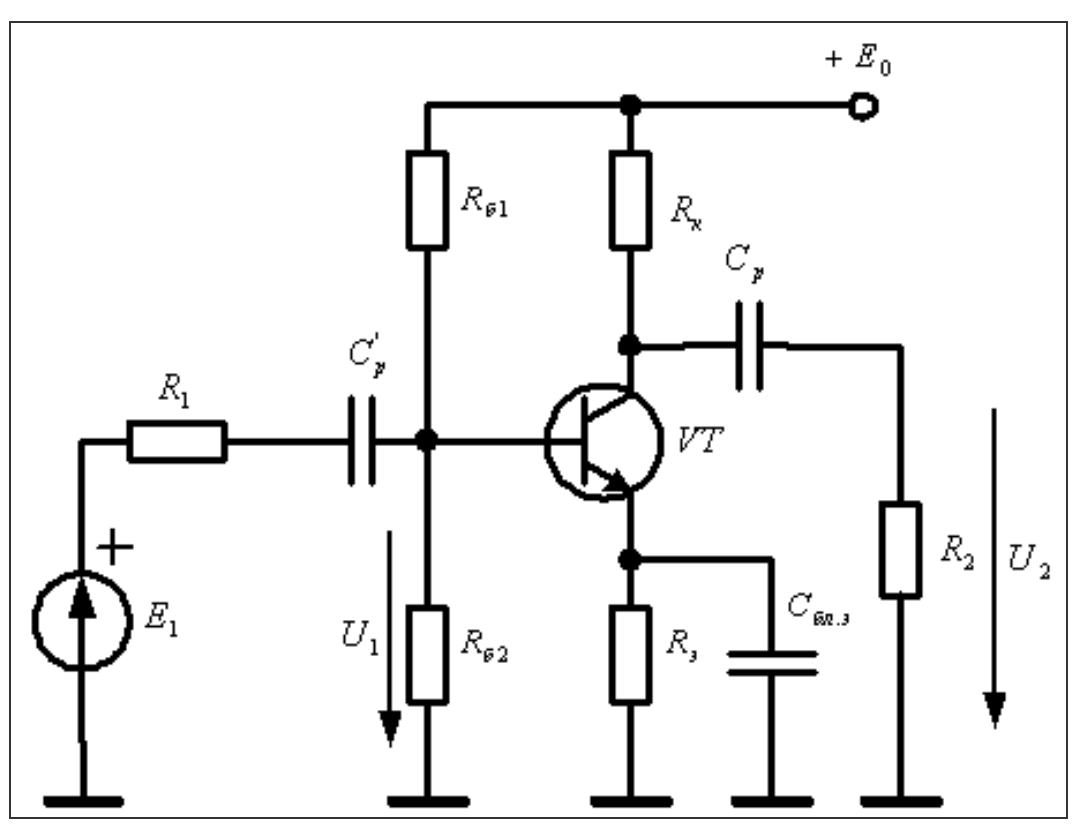
\includegraphics[scale=0.2]{oe.png}}
                \caption{Могут ли каскады ОЭ, ОБ,ОК иметь одинаковые большую верхнюю граничную частоту}
        \end{figure}
\end{center}

берем из 11 вопроса все, кроме того, что касается ОК. Из табл видно, что совпадают


